\documentclass[tikz,border=3pt]{standalone}
% Shared style for every figure: one font (Latin Modern), one block vocabulary, token colours.
\usepackage{fontspec}
\usepackage{unicode-math}
\setmathfont{latinmodern-math.otf}
\usetikzlibrary{arrows.meta,positioning,fit,calc,backgrounds,shapes.misc,decorations.pathreplacing}
% Token colours: exact RGB codes, remapped to CSS variables after conversion (see tokens in svgfix.py)
\definecolor{ink}{RGB}{0,0,0}
\definecolor{inkb}{RGB}{90,90,90}
\definecolor{grid}{RGB}{200,200,200}
\definecolor{paper}{RGB}{255,255,255}
\definecolor{fdata}{RGB}{231,238,246}
\definecolor{fmodel}{RGB}{246,238,224}
\definecolor{ftarget}{RGB}{232,243,234}
\definecolor{fpub}{RGB}{248,233,226}
\definecolor{own}{RGB}{42,120,214}
\definecolor{pub}{RGB}{235,104,52}
\tikzset{
  >={Latex[length=1.9mm,width=1.5mm]},
  every picture/.style={line width=0.5pt, ink, font=\normalsize},
  blk/.style={draw=ink, rounded corners=1.2pt, align=center, inner xsep=5pt, inner ysep=4pt, minimum height=9mm, fill=paper},
  data/.style={blk, fill=fdata},
  model/.style={blk, fill=fmodel},
  target/.style={blk, fill=ftarget},
  pubm/.style={blk, fill=fpub},
  op/.style={draw=ink, circle, inner sep=1.2pt, fill=paper, font=\small},
  group/.style={draw=inkb, dashed, rounded corners=2pt, inner sep=6pt},
  glabel/.style={font=\small\scshape, text=inkb, inner sep=1pt},
  note/.style={font=\footnotesize, text=inkb, align=center, inner sep=1pt},
  wt/.style={font=\footnotesize, fill=paper, inner sep=1pt},
  flow/.style={->, draw=ink},
  dflow/.style={->, draw=inkb, dashed},
}

\begin{document}
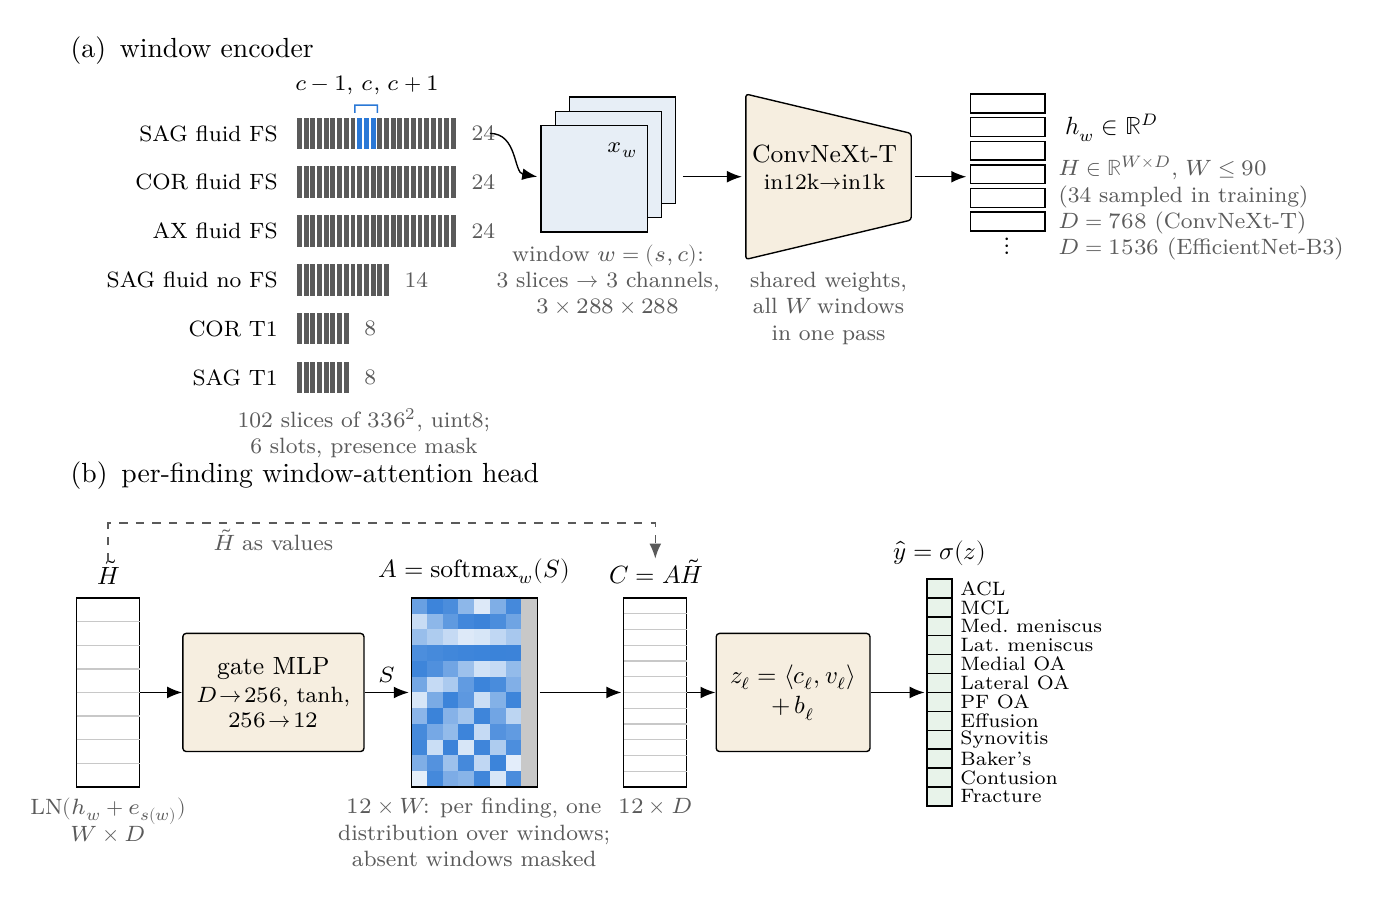
\begin{tikzpicture}[font=\small]
% ---------------- panel (a): study tensor -> windows -> encoder -> tokens ----------------
\node[anchor=west, font=\normalsize] at (-3.0,2.55) {(a)\enspace window encoder};
% slot stacks: slices drawn as thin bars, 0.085 cm pitch
\def\pitch{0.085}
\foreach \name/\n/\row in {SAG fluid FS/24/0, COR fluid FS/24/1, AX fluid FS/24/2, SAG fluid no FS/14/3, COR T1/8/4, SAG T1/8/5}{
  \pgfmathsetmacro{\y}{1.5-0.62*\row}
  \node[anchor=east, font=\footnotesize] at (-0.12,\y) {\name};
  \foreach \i in {1,...,\n}{
    \fill[inkb] ({(\i-1)*\pitch},{\y-0.2}) rectangle ++(0.062,0.4);
  }
  \node[anchor=west, font=\footnotesize, text=inkb] at ({\n*\pitch+0.05},\y) {\n};
}
% highlighted window in the first slot: slices 10, 11, 12
\foreach \i in {10,11,12}{ \fill[own] ({(\i-1)*\pitch},1.3) rectangle ++(0.062,0.4); }
\draw[own, line width=0.5pt] ({9*\pitch-0.03},1.76) -- ++(0,0.1) -- ({12*\pitch+0.0},1.86) -- ++(0,-0.1);
\node[font=\footnotesize, text=ink, anchor=south] at ({10.5*\pitch},1.86) {$c-1,\,c,\,c+1$};
\node[note, anchor=north] at (0.85,-1.95) {102 slices of $336^2$, uint8;\\6 slots, presence mask};
% window triplet
\begin{scope}[shift={(3.1,0.25)}]
  \foreach \k in {2,1,0}{
    \filldraw[fill=fdata, draw=ink] ({0.18*\k},{0.18*\k}) rectangle ++(1.35,1.35);
  }
  \node[font=\footnotesize] at (0.675+0.36,0.675+0.36) {$x_w$};
  \node[note, anchor=north, align=center] at (0.85,-0.12) {window $w=(s,c)$:\\3 slices $\to$ 3 channels,\\$3\times288\times288$};
\end{scope}
\draw[flow] (2.45,1.5) .. controls (2.8,1.5) and (2.75,1.0) .. (3.05,0.95);
% encoder trapezoid
\begin{scope}[shift={(5.7,0.95)}]
  \filldraw[fill=fmodel, draw=ink, rounded corners=1pt] (0,-1.05) -- (2.1,-0.55) -- (2.1,0.55) -- (0,1.05) -- cycle;
  \node[align=center] at (1.0,0.12) {ConvNeXt-T\\[-1pt]\footnotesize in12k$\to$in1k};
  \node[note, anchor=north, align=center] at (1.05,-1.17) {shared weights,\\all $W$ windows\\in one pass};
\end{scope}
\draw[flow] (4.9,0.95) -- (5.65,0.95);
% token column H
\begin{scope}[shift={(8.55,0.95)}]
  \foreach \j in {0,...,5}{ \filldraw[fill=paper, draw=ink] (0,{1.05-0.3*\j}) rectangle ++(0.95,-0.24); }
  \node at (0.475,-0.88) {$\vdots$};
  \node[anchor=west, align=left] at (1.08,0.62) {$h_w\in\mathbb{R}^{D}$};
  \node[note, anchor=north west, align=left] at (1.08,0.3) {$H\in\mathbb{R}^{W\times D}$, $W\le 90$\\(34 sampled in training)\\$D=768$ (ConvNeXt-T)\\$D=1536$ (EfficientNet-B3)};
\end{scope}
\draw[flow] (7.85,0.95) -- (8.5,0.95);
% ---------------- panel (b): per-finding window attention head ----------------
\begin{scope}[shift={(0,-5.6)}]
\node[anchor=west, font=\normalsize] at (-3.0,2.75) {(b)\enspace per-finding window-attention head};
% H tilde
\filldraw[fill=paper, draw=ink] (-2.8,-1.2) rectangle (-2.0,1.2);
\foreach \j in {1,...,7}{ \draw[grid] (-2.8,{-1.2+0.3*\j}) -- (-2.0,{-1.2+0.3*\j}); }
\node[anchor=south] at (-2.4,1.25) {$\tilde H$};
\node[note, anchor=north, align=center] at (-2.4,-1.3) {$\mathrm{LN}(h_w+e_{s(w)})$\\$W\times D$};
% gate MLP
\node[model, minimum width=2.15cm, minimum height=1.5cm] (gate) at (-0.3,0) {gate MLP\\[-1pt]\footnotesize $D\!\to\!256$, tanh,\\[-2pt]\footnotesize $256\!\to\!12$};
\draw[flow] (-2.0,0) -- (gate.west);
% score / attention grids (12 rows x 8 window columns, last column = padded window)
\def\cw{0.2}
\begin{scope}[shift={(1.45,-1.2)}]
  \foreach \r in {0,...,11}{ \foreach \c in {0,...,7}{
    \pgfmathsetmacro{\op}{0.12+0.8*abs(sin(37*\r+71*\c+13*\r*\c))}
    \ifnum\c=7 \fill[grid] ({\c*\cw},{\r*\cw}) rectangle ++(\cw,\cw);
    \else \fill[own, fill opacity=\op] ({\c*\cw},{\r*\cw}) rectangle ++(\cw,\cw); \fi
  }}
  \draw[ink, line width=0.4pt] (0,0) rectangle ({8*\cw},{12*\cw});
  \node[anchor=south] at ({4*\cw},{12*\cw+0.05}) {$A=\mathrm{softmax}_w(S)$};
  \node[note, anchor=north, align=center] at ({4*\cw},-0.1) {$12\times W$: per finding, one\\distribution over windows;\\absent windows masked};
\end{scope}
\draw[flow] (gate.east) -- node[above, font=\footnotesize] {$S$} (1.42,0);
% context
\filldraw[fill=paper, draw=ink] (4.15,-1.2) rectangle (4.95,1.2);
\foreach \j in {1,...,11}{ \draw[grid] (4.15,{-1.2+0.2*\j}) -- (4.95,{-1.2+0.2*\j}); }
\node[anchor=south] at (4.55,1.25) {$C=A\tilde H$};
\node[note, anchor=north] at (4.55,-1.3) {$12\times D$};
\draw[flow] (3.08,0) -- (4.12,0);
\draw[dflow] (-2.4,1.66) -- (-2.4,2.15) -- (4.55,2.15) -- (4.55,1.7);
\node[note, anchor=north] at (-0.3,2.12) {$\tilde H$ as values};
% per-finding readout
\node[model, minimum width=1.75cm, minimum height=1.5cm] (ro) at (6.3,0) {$z_\ell=\langle c_\ell, v_\ell\rangle$\\$+\,b_\ell$};
\draw[flow] (4.95,0) -- (ro.west);
% logits list
\begin{scope}[shift={(8.0,-1.44)}]
  \foreach \lab [count=\r from 0] in {Fracture,Contusion,Baker's,Synovitis,Effusion,PF OA,Lateral OA,Medial OA,Lat.\ meniscus,Med.\ meniscus,MCL,ACL}{
    \filldraw[fill=ftarget, draw=ink] (0,{\r*0.24}) rectangle ++(0.32,0.24);
    \node[anchor=west, font=\scriptsize, inner sep=1pt] at (0.38,{\r*0.24+0.12}) {\lab};
  }
  \node[anchor=south] at (0.16,2.92) {$\hat y=\sigma(z)$};
\end{scope}
\draw[flow] (ro.east) -- (7.97,0);
\end{scope}
\end{tikzpicture}
\end{document}
